%++++++++++++++++++++++++++++++++++++++++
% Don't modify this section unless you know what you're doing!
\documentclass[letterpaper,12pt, dvipsnames, dateno]{article}
\usepackage{tabularx} % extra features for tabular environment
\usepackage{amsmath}  % improve math presentation
\usepackage{graphicx} % takes care of graphic including machinery
\usepackage[margin=1in,letterpaper]{geometry} % decreases margins
\usepackage{cite} % takes care of citations
\usepackage[final]{hyperref} % adds hyper links inside the generated pdf file
\usepackage{enumitem}
\usepackage{graphicx}
\usepackage{listings}

% color boxes
\usepackage{tikz,lipsum,lmodern}
\usepackage[most]{tcolorbox}
\tcbuselibrary{listings,breakable}

% diacritice
\usepackage[utf8]{inputenc}


% code listing Python
\lstset{language=Python}
\lstset{frame=lines}
\lstset{label={lst:code_direct}}
% \lstset{basicstyle=\footnotesize}

\usepackage[english, romanian]{babel}
\usepackage{combelow}

% \usepackage{newunicodechar}
% \newunicodechar{Ș}{\cb{S}}
% \newunicodechar{ș}{\cb{s}}
% \newunicodechar{Ț}{\cb{T}}
% \newunicodechar{ț}{\cb{t}}
% \newunicodechar{ă}{\u{a}}

% \newunicodechar{Î}{\^{i}}
% \newunicodechar{î}{\^{i}}

\newtcbox{\mybox}[2][]{nobeforeafter,tcbox raise base,colframe=#2,colback=#2!10!white,top=0.8pt,bottom=0.8pt, left=0.8pt, right=0.8pt,before upper=\strut}

% part of speech tagging
\newtcbox{\pstag}[2][]{nobeforeafter,tcbox raise base,colframe=#2,colback=#2,top=0.8pt,bottom=0.8pt, left=0.8pt, right=0.8pt,before upper=\strut}
\hypersetup{
	colorlinks=true,       % false: boxed links; true: colorend links
	linkcolor=black,        % color of internal links
	citecolor=blue,        % color of links to bibliography
	filecolor=magenta,     % color of file links
	urlcolor=blue         
}
%++++++++++++++++++++++++++++++++++++++++

% \def\abstractname{{\it Abstract}}

\begin{document}

\title{NeuralCoref: Coreference Resolution in spaCy}
\author{Dana Nica 341C4}
\date{}
\maketitle


% \tableofcontents

% \begin{abstract}

% \end{abstract}


\section{Introducere}
În lingvistică, coreferința, apare atunci când 2 sau mai multe expresii dintr-un text referă aceeași persoană sau același obiect, cu alte cuvinte au același referent. Rezoluția coreferințelor este procesul de asociere a mențiunilor care referă aceeași entitate. \\

\textit{Exemplu:} "When \mybox{ForestGreen}{Emily \pstag{ForestGreen}{\scriptsize PROPER}} is at the front door, \mybox{ForestGreen}{she \pstag{ForestGreen}{\scriptsize PRONOMINAL}} must be leaving the house" \\ \\
Substantivul propriu \textit{Emily} și pronumele \textit{she} referă aceeași persoană- Emily.\\

\textbf{Tipuri de coreferințe}
\begin{itemize}
    \item{\textbf{Anaphora} (anaphora presupune folosirea unei expresii care depinde de o expresie specifică anterioară) \\
    "Because \mybox{Salmon}{David \pstag{Salmon}{\scriptsize PROPER}} was so cold, \mybox{Salmon}{he \pstag{Salmon}{\scriptsize PRONOMINAL}} put on \mybox{Salmon}{his \pstag{Salmon}{\scriptsize PRONOMINAL}} coat." \\ \\
    "\mybox{Purple}{My sister \pstag{Purple}{\scriptsize NOMINAL}} has \mybox{YellowOrange}{a dog \pstag{YellowOrange}{\scriptsize NOMINAL}}. \mybox{Purple}{She \pstag{Purple}{\scriptsize PRONOMINAL}} loves \mybox{YellowOrange}{him \pstag{YellowOrange}{\scriptsize PRONOMINAL}}." 
    }
    \item{\textbf{Cataphora} (folosirea unei expresii sau a unui cuvânt care referă o expresie ulterioară, mai specifică, în discurs) \\ \\
    "Because \mybox{Salmon}{he \pstag{Salmon}{\scriptsize PRONOMINAL}} was so cold, \mybox{Salmon}{David \pstag{Salmon}{\scriptsize PROPER}} put on \mybox{Salmon}{his \pstag{Salmon}{\scriptsize PRONOMINAL}} coat." \\ \\
    "\mybox{SeaGreen}{His \pstag{SeaGreen}{\scriptsize PRONOMINAL}} friends have been criticizing \mybox{SeaGreen}{Jim \pstag{SeaGreen}{\scriptsize PROPER}} for exaggerating."
    }
    \item{\textbf{Split antecedents}\\ \\
    "\mybox{GreenYellow}{Carol \pstag{GreenYellow}{\scriptsize PROPER}} told \mybox{GreenYellow}{Bob \pstag{GreenYellow}{\scriptsize PROPER}} to attend the party. \mybox{GreenYellow}{They \pstag{GreenYellow}{\scriptsize PRONOMINAL}} arrived together." \\ \\
     They referă atât pe Bob cât și pe Carol.
    }
    \item{\textbf{Coreferring noun phrases} \\ \\
    "\mybox{YellowGreen}{Some of our colleagues \pstag{YellowGreen}{\scriptsize NOMINAL}} are going to be supportive. \mybox{YellowGreen}{These kinds of people \pstag{YellowGreen}{\scriptsize NOMINAL}} will earn our gratitude."}
\end{itemize}
    


\section{NeuralCoref}
NeuralCoref[3] este o bibliotecă open source, integrată ca o extensie pipeline în spaCy 2.0 care adnotează și rezolvă coreferințele folosind o rețea neurală.  Pentru a folosi NeuralCoref, se incarcă modelul descarcat  și se procesează textul cu spaCy. NeuralCoref rezolvă coreferințele și le adnotează ca atribute ale obiectelor spaCy Doc, Span si Token  sub dicționarul  .\_. 
Exista posibilitatea de a reantrena un model, sau de a extinde la o altă limbă.[5][6]\\

\selectlanguage{romanian}

\begin{figure}[ht]
    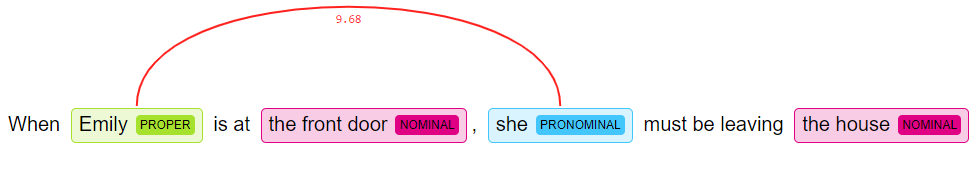
\includegraphics[scale=0.70]{exemplu-coref2.PNG}
    \caption{Obținută cu NeuralCoref-Viz[2]}
    \label{fig:my_label}
\end{figure}

\selectlanguage{romanian}

\lstset{caption={Rezolvarea coreferințelor}}
\begin{lstlisting}[showstringspaces=false]
import spacy
nlp = spacy.load('en_coref_sm')

coref = "When Emily is at the front door, she must be leaving the house"
resolved_coref = nlp(coref).doc._.coref_resolved

print(resolved_coref)
\end{lstlisting}
% \lstinputlisting[language=Python]{mesh.py}


\begin{verbatim}
When Emily is at the front door, Emily must be leaving the house.
\end{verbatim}

\section{Concluzii}
NeuralCoref rezolvă doar coreferințele de tipul anaphora. Pentru celelalte cazuri nu identifică complet(Figura 2) sau corect(Figura 3, 4) coreferințele.

\begin{figure}[ht]
    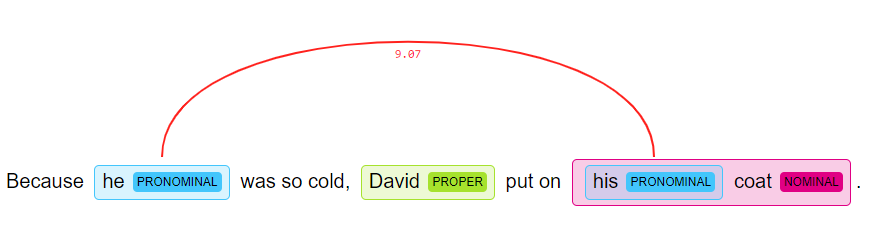
\includegraphics[scale=0.70]{coref1.PNG}
    \caption{Obținută cu NeuralCoref-Viz[2]}
    \label{fig:my_label}
\end{figure}

\begin{figure}[ht]
    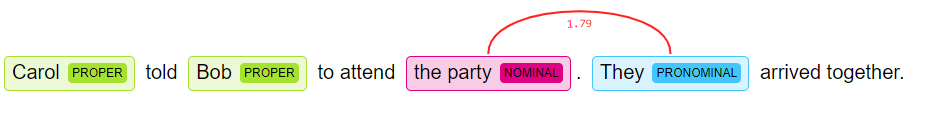
\includegraphics[scale=0.70]{coref2.PNG}
    \caption{Obținută cu NeuralCoref-Viz[2]}
    \label{fig:my_label}
\end{figure}

\begin{figure}[ht]
    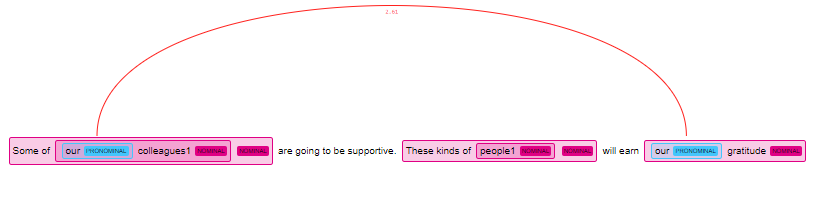
\includegraphics[scale=0.70]{coref3.PNG}
    \caption{Obținută cu NeuralCoref-Viz[2]}
    \label{fig:my_label}
\end{figure}

În anexa A sunt prezentate scenarii de utilizare ce conțin coreferințe, iar în anexa B sunt prezentate rezultatele obținute folosind NeuralCoref pe întreaga conversație, informație deținută de agent a fost analizată separat. 

\selectlanguage{romanian}
\begin{thebibliography}{99}

\bibitem{melissinos} \href{https://spacy.io/usage/spacy-101}{spaCy 101}

\bibitem{melissinos} NeuralCoref is accompanied by a visualization client  \href{https://huggingface.co/coref/}{NeuralCoref-Viz}

\bibitem{melissinos} \href{https://github.com/huggingface/neuralcoref}{NeuralCoref: Coreference Resolution în spaCy with Neural Networks}

\bibitem{melissinos} \href{https://bit.ly/2DMo8RP}{State-of-the-art neural coreference resolution for chatbots}

\bibitem{melissinos} \href{https://bit.ly/2DWBcAT}{How to train a neural coreference model— Neuralcoref 2}

\bibitem{melissinos} \href{https://github.com/huggingface/neuralcoref/blob/master/neuralcoref/train/training.md}{How to train and modify the neural coreference model}


\end{thebibliography}

\section{Anexă A - Scenarii de utilizare }

\textbf{\textit{Legendă: I = informație deținută de agent U = Cerere adresată de utilizator A = răspunsul agentului}}


\begin{enumerate}[label=\textbf{\arabic*}]
    \item{ I: Mrs. \mybox{WildStrawberry}{\mybox{YellowGreen}{Robinson \pstag{YellowGreen}{\scriptsize PROPER}}'s phone \pstag{WildStrawberry}{\scriptsize NOMINAL}} is 0725555566, \mybox{WildStrawberry}{her \pstag{WildStrawberry}{\scriptsize PRONOMINAL}} office room is 236. \mybox{WildStrawberry}{She \pstag{WildStrawberry}{\scriptsize PRONOMINAL}} will attend the AI Conference in Bucharest on 20th  February 2019. Today is 19th February 2019. \\ \\
           U: What is the telephone number of Msr. Robinson ? \\ \\
           A: The telephone number of \mybox{DarkOrchid}{Msr. Robinson \pstag{DarkOrchid}{\scriptsize PROPER}} is 0725555566.\\ \\
           U: What about \mybox{DarkOrchid}{her \pstag{DarkOrchid}{\scriptsize PRONOMINAL}} office room?\\ \\
           A: \mybox{DarkOrchid}{Her \pstag{DarkOrchid}{\scriptsize PRONOMINAL}} office room is 236.\\ \\
           U: Will \mybox{DarkOrchid}{she \pstag{DarkOrchid}{\scriptsize PRONOMINAL}} attend the \mybox{SeaGreen}{AI Conference \pstag{SeaGreen}{\scriptsize NOMINAL}} tomorrow afternoon?\\ \\
           A: Yes,  \mybox{DarkOrchid}{she \pstag{DarkOrchid}{\scriptsize PRONOMINAL}} will.\\ \\
           U: Where will  \mybox{SeaGreen}{it \pstag{SeaGreen}{\scriptsize PRONOMINAL}} take place?\\ \\
           A: \mybox{SeaGreen}{It \pstag{SeaGreen}{\scriptsize PRONOMINAL}} will take place in Bucharest.
           }
    
    \item{
        I: \mybox{Dandelion}{My dog \pstag{Dandelion}{\scriptsize NOMINAL}}'s name is Sudo. \mybox{Dandelion}{Him \pstag{Dandelion}{\scriptsize PRONOMINAL} } has to be fed in the morning and in the evening. \\ \\
        U: What's \mybox{Mahogany}{my dog \pstag{Mahogany}{\scriptsize NOMINAL}}'s name? \\ \\
        A: \mybox{Mahogany}{His \pstag{Mahogany}{\scriptsize PRONOMINAL}} name is Sudo. \\ \\ 
        U: When do I have to fed \mybox{Mahogany}{him \pstag{Mahogany}{\scriptsize PRONOMINAL}}? \\ \\
        A: In the morning and in the evening.
        
    
    } 
    \item{
        I: On Monday I am meeting \mybox{NavyBlue}{Andreea \pstag{NavyBlue}{\scriptsize PROPER}}. \mybox{NavyBlue}{She \pstag{NavyBlue}{\scriptsize PRONOMINAL}} will borrow me a book.\\ \\
        U: Who am I meeting on Monday? \\ \\
        A: You will be meeting  \mybox{PineGreen}{Andreea \pstag{PineGreen}{\scriptsize PROPER}}. \\ \\
        U: What will \mybox{PineGreen}{She \pstag{PineGreen}{\scriptsize PRONOMINAL}} borrow me? \\ \\
        A: \mybox{PineGreen}{She \pstag{PineGreen}{\scriptsize PRONOMINAL}} will borrow you a book.
        
    } 
    \item{
        I: \mybox{Plum}{A good movie \pstag{Plum}{\scriptsize NOMINAL}} is Bohemian Rhapsody.\mybox{Plum}{It \pstag{Plum}{\scriptsize PRONOMINAL}} was directed by Bryan Singer. \mybox{Goldenrod}{Rami Malek \pstag{Goldenrod}{\scriptsize PROPER}} plays Freddie Mercury in the movie and \mybox{Goldenrod}{he \pstag{Goldenrod}{\scriptsize PRONOMINAL}} won an Oscar for Best Actor.\\ \\
        U: Recommend me a good movie. \\ \\
        A: \mybox{CornflowerBlue}{A good movie \pstag{CornflowerBlue}{\scriptsize NOMINAL}} is Bohemian Rhapsody. \\ \\
        U: Who directed \mybox{CornflowerBlue}{it \pstag{CornflowerBlue}{\scriptsize PRONOMINAL}}? \\ \\
        A: Bryan Singer directed \mybox{CornflowerBlue}{it \pstag{CornflowerBlue}{\scriptsize PRONOMINAL}}.\\ \\ 
        U: Who plays Freddie Mercury in the movie? \\ \\ 
        A: \mybox{Rhodamine}{Rami Malek \pstag{Rhodamine}{\scriptsize PROPER}} plays Freddie Mercury in the movie. \\ \\
        U: Did \mybox{Rhodamine}{he \pstag{Rhodamine}{\scriptsize PRONOMINAL}} win an Oscar? \\ \\
        A: Yes, \mybox{Rhodamine}{he \pstag{Rhodamine}{\scriptsize PRONOMINAL}} won an Oscar for best actor.
    }
           
    \item{
         I: Tomorrow I have a Machine Learning course from 9 am to 11 am. \\ \\
         U: Set an alarm at 8 am. \\ \\
         A: Alarm set. \\ \\
         U: What course do I have tomorrow? \\ \\
         A: You have \mybox{OliveGreen}{\mybox{Thistle}{a Machine Learning \pstag{Thistle}{\scriptsize PROPER}} course \pstag{OliveGreen}{\scriptsize NOMINAL}}. \\
         
         U: When will \mybox{OliveGreen}{the course \pstag{OliveGreen}{\scriptsize NOMINAL}} start? \\
         A: \mybox{OliveGreen}{It \pstag{OliveGreen}{\scriptsize PRONOMINAL}} will start at 9 am. \\
         U: How many hours does \mybox{OliveGreen}{it \pstag{OliveGreen}{\scriptsize PRONOMINAL}} last? \\
         A: \mybox{OliveGreen}{It \pstag{OliveGreen}{\scriptsize PRONOMINAL}} lasts 2 hours.
    }
    \\ \\
    \item{
        I: \mybox{SkyBlue}{Sherlock \pstag{SkyBlue}{\scriptsize PROPER}} is a British crime drama television series based on Sir Arthur Conan Doyle's Sherlock Holmes detective stories. Created by Steven Moffat and Mark Gatiss, \mybox{SkyBlue}{it \pstag{SkyBlue}{\scriptsize PRONOMINAL}} stars Benedict Cumberbatch as Sherlock Holmes and Martin Freeman as Doctor John Watson. Thirteen episodes have been produced, with four three-part series airing from 2010 to 2017, and a special episode that aired on 1 January 2016. \\ \\ \\
        I: \mybox{CarnationPink}{Criminal Minds \pstag{CarnationPink}{\scriptsize PROPER}} is an American police procedural crime drama television series created and produced by Jeff Davis. \mybox{CarnationPink}{It \pstag{CarnationPink}{\scriptsize PRONOMINAL}} premiered on September 22, 2005, and has run for fourteen seasons on CBS. \mybox{CarnationPink}{It \pstag{CarnationPink}{\scriptsize PRONOMINAL}} tells the story of a group of behavioral profilers who work for \mybox{RedOrange}{the FBI \pstag{RedOrange}{\scriptsize PROPER} } as members of \mybox{RedOrange}{its  \pstag{RedOrange}{\scriptsize PRONOMINAL}} Behavioral Analysis Unit (BAU). \\ \\ \\
        U: Recommend me a crime television series. \\ \\
        A: \mybox{Goldenrod}{\mybox{YellowGreen}{Sherlock \pstag{YellowGreen}{\scriptsize PROPER}} and \mybox{YellowGreen}{Criminal Minds \pstag{YellowGreen}{\scriptsize PROPER}} \pstag{Goldenrod}{\scriptsize LIST}} are crime television series. \\ \\
        U: Which one of \mybox{Goldenrod}{them \pstag{Goldenrod}{\scriptsize PRONOMINAL}} is a British television series? \\ \\
        A: \mybox{Green}{Sherlock \pstag{Green}{\scriptsize PROPER}} is a British television series. \\ \\
        U: Who stars in \mybox{Green}{it \pstag{Green}{\scriptsize PRONOMINAL}} ? \\ \\
        A: Benedict Cumberbatch stars in \mybox{Green}{it \pstag{Green}{\scriptsize PRONOMINAL}} . 
    }

\end{enumerate}

\section{Anexă B - Rezultate obținute folosind NeuralCoref}
\begin{enumerate}[label=\textbf{\arabic*}]
  
    \item{
    Coreferințe identificate:\\ \\
    I: [Mrs. Robinson's phone: [Mrs. Robinson's phone, her, She]] \\
    CONV: [Mrs. Robinson: [Mrs. Robinson, Her, her, Her, she, she], her office room: [her office room, Her office room]]
    \\
    Coreferințe neidentificate: \\ \\
    What is the telephone number of Mrs. Robinson? Her phone number is 0725555566. What about her office room? Her office room is 236.Will she attend the \mybox{SeaGreen}{AI Conference \pstag{SeaGreen}{\scriptsize NOMINAL}} tomorrow afternoon?Yes,  she will.Where will  \mybox{SeaGreen}{it \pstag{SeaGreen}{\scriptsize PRONOMINAL}} take place? \mybox{SeaGreen}{It \pstag{SeaGreen}{\scriptsize PRONOMINAL}} will take place In Bucharest.
    }
    
    \item{
    Coreferințe identificate:\\ \\
    I: [My dog's name: [My dog's name, He]] \\ \\
    CONV: [my dog's name: [my dog's name, His name], His: [His, him]]\\ \\
    Coreferințe neidentificate: - \\ \\
    }
    
    \item{
    Coreferințe identificate:\\ \\
    I: [Andreea: [Andreea, She]]\\ \\
    CONV: [Andreea: [Andreea, she, She]]\\ \\
    Coreferințe neidentificate: - \\ \\
    }
    
  
    
    \item{
    Coreferințe identificate:\\ \\
    I: [A good movie: [A good movie, It, the movie], Rami Malek: [Rami Malek, he]]\\ \\
    CONV: [A good movie: [A good movie, the movie, the movie], it: [it, it], Freddie Mercury: [Freddie Mercury, Freddie Mercury], Rami Malek: [Rami Malek, he, he]]\\ \\
    Coreferințe neidentificate:\\ \\
    \mybox{CornflowerBlue}{A good movie \pstag{CornflowerBlue}{\scriptsize NOMINAL}} is Bohemian Rhapsody. Who directed \mybox{CornflowerBlue}{it \pstag{CornflowerBlue}{\scriptsize PRONOMINAL}}? Bryan Singer directed \mybox{CornflowerBlue}{it \pstag{CornflowerBlue}{\scriptsize PRONOMINAL}}.
    }
    
     \item{
    Coreferințe identificate:\\ \\
    I: -\\ \\
    CONV: [a Machine Learning course: [a Machine Learning course, the course, It, it, It]]\\ \\
    Coreferințe neidentificate: - \\ \\
    }
    
    \item{
    Coreferințe identificate:\\ \\
    I: [Sherlock: [Sherlock, it]]\\ \\
    I: [Criminal Minds: [Criminal Minds, It, It], the FBI: [the FBI, its]]\\ \\
    CONV: [Sherlock and Criminal Minds: [Sherlock and Criminal Minds, them], Sherlock: [Sherlock, it, it]]\\ \\
    Coreferințe neidentificate: - \\ \\
    }
    
    
    
    
\end{enumerate}
\end{document}